\documentclass[tikz,border=8pt]{standalone}
% Shared look for every TikZ diagram. Load with \input{../../tools/tikz-style.tex}
\usepackage[sfdefault]{roboto}
\usetikzlibrary{arrows.meta, positioning, shapes.geometric, calc, fit, backgrounds}
\definecolor{cblue}{HTML}{4C78A8}
\definecolor{corange}{HTML}{F58518}
\definecolor{cgreen}{HTML}{54A24B}
\definecolor{cred}{HTML}{E45756}
\definecolor{cpurple}{HTML}{B279A2}
\definecolor{cgrey}{HTML}{6B6B6B}
\tikzset{
  every picture/.style={font=\sffamily, line width=1.2pt},
  box/.style={draw=#1, fill=#1!12, rounded corners=4pt, align=center, inner sep=7pt, minimum height=1.1cm},
  box/.default=cgrey,
  arrow/.style={-{Stealth[length=3mm]}, draw=cgrey, line width=1.4pt},
  title/.style={font=\sffamily\bfseries\Large},
  note/.style={font=\sffamily\small, text=cgrey, align=center},
}
\AtBeginDocument{\hyphenpenalty=10000 \exhyphenpenalty=10000}

% The heading cascade: the outer loop turns the heading error into a yaw-rate command (gain 1 per s, capped at
% 1 rad/s); the inner loop turns the yaw-rate error, measured by the gyro, into torque (PI, limited to 0.2 N m).
% The robot's yaw inertia turns torque into yaw rate, and yaw rate adds up to heading.
\begin{document}
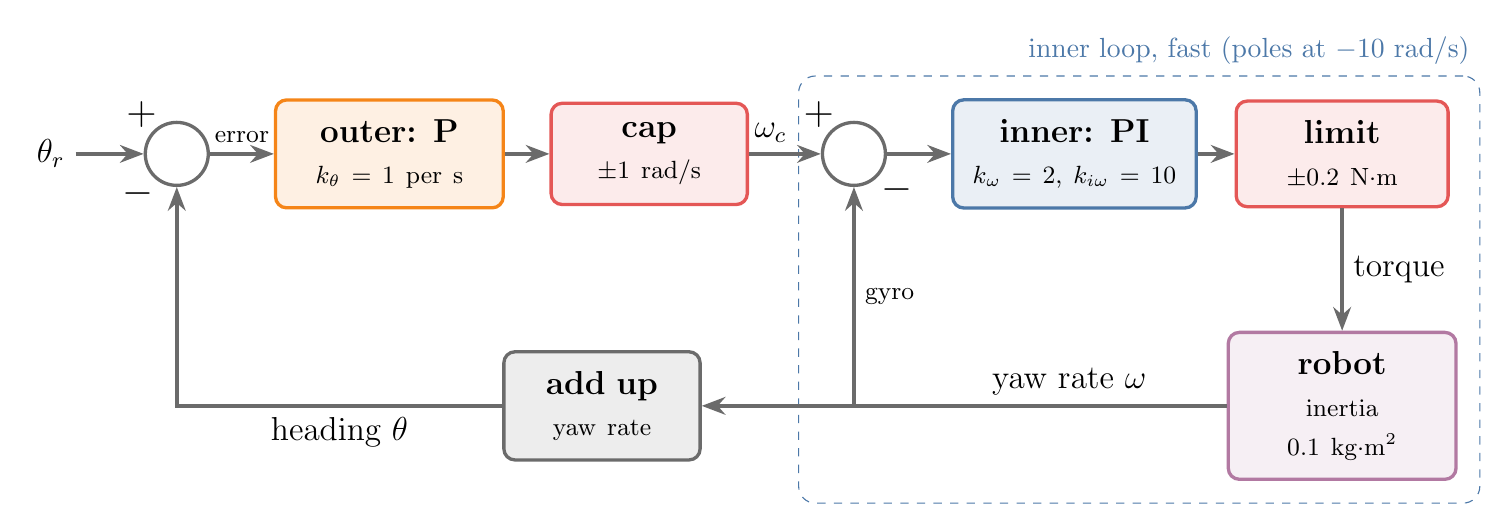
\begin{tikzpicture}[every node/.append style={font=\large}]
  \node (r) at (0,0) {$\theta_r$};
  \node[circle, draw=cgrey, fill=white, minimum size=0.8cm, inner sep=0pt] (s1) at (1.6,0) {};
  \node[box=corange, text width=2.4cm] (outer) at (4.3,0) {\textbf{outer: P}\\[1pt] \small $k_\theta$ = 1 per s};
  \node[box=cred, text width=2.0cm] (cap) at (7.6,0) {\textbf{cap}\\[1pt] \small $\pm$1 rad/s};
  \node[circle, draw=cgrey, fill=white, minimum size=0.8cm, inner sep=0pt] (s2) at (10.2,0) {};
  \node[box=cblue, text width=2.6cm] (inner) at (13.0,0) {\textbf{inner: PI}\\[1pt] \small $k_\omega$ = 2, $k_{i\omega}$ = 10};
  \node[box=cred, text width=2.2cm] (lim) at (16.4,0) {\textbf{limit}\\[1pt] \small $\pm$0.2 N$\cdot$m};
  \node[box=cpurple, text width=2.4cm] (body) at (16.4,-3.2) {\textbf{robot}\\[1pt] \small inertia 0.1 kg$\cdot$m$^2$};
  \node[box=cgrey, text width=2.0cm] (add) at (7.0,-3.2) {\textbf{add up}\\[1pt] \small yaw rate};
  \draw[arrow] (r) -- (s1);
  \node[font=\Large] at ($(s1.north west)+(-0.15,0.2)$) {$+$};
  \draw[arrow] (s1) -- node[above] {\small error} (outer);
  \draw[arrow] (outer) -- (cap);
  \draw[arrow] (cap) -- node[pos=0.3, above] {$\omega_c$} (s2);
  \node[font=\Large] at ($(s2.north west)+(-0.15,0.2)$) {$+$};
  \draw[arrow] (s2) -- (inner);
  \draw[arrow] (inner) -- (lim);
  \draw[arrow] (lim) -- node[right] {torque} (body);
  \draw[arrow] (body) -- node[pos=0.3, above] {yaw rate $\omega$} (add);
  \draw[arrow] (s2 |- body.west) -- node[pos=0.5, right] {\small gyro} (s2.south);
  \node[font=\Large] at ($(s2.south east)+(0.25,-0.15)$) {$-$};
  \draw[arrow] (add.west) -| node[pos=0.25, below] {heading $\theta$} (s1.south);
  \node[font=\Large] at ($(s1.south west)+(-0.2,-0.2)$) {$-$};
  \begin{scope}[on background layer]
    \node[draw=cblue, dashed, rounded corners=6pt, inner sep=8pt, fit=(s2) (inner) (lim) (body)] (il) {};
  \end{scope}
  \node[note, font=\normalsize, text=cblue, anchor=south east] at (il.north east) {inner loop, fast (poles at $-$10 rad/s)};
\end{tikzpicture}
\end{document}
